% command to make sure colorboxes don't create whitespace between code lines
\fboxsep=.6pt

% default settings for listings

\lstset{style=Python, basicstyle=\scriptsize\ttfamily,escapechar=!}

\begin{frame}
	\centering
	\begin{figure}[H]
		\includegraphics[keepaspectratio, width=0.7\paperwidth, height=\paperheight]{\thelogo}
	\end{figure}
	Informatik: Programmieren\\
	\emoji{turtle} Kapitel 01: \textbf{Einführung}
\end{frame}

\begin{frame}{Einführung}
	Was erwartet Sie?
	\begin{itemize}
		\item \textbf{Programmieren}: Grundkonzepte (Schleifen, Verzweigungen, Variablen)
		\item \textbf{Robotik}: Steuerung von Technik (Roboter, Sensoren, Aktoren)
	\end{itemize}
\end{frame}



\begin{frame}[fragile]{Lehrmittel: Skript}
	\begin{columns}[c]
	\centering
		\begin{column}{.4\linewidth}
			\begin{figure}[H]
				\centering
				
\includegraphics[width=\columnwidth]{"GrundlagenInfo/00_Programmieren/Figures/Programmieren Skript Title Page.pdf"}
			\end{figure}
		\end{column}

		\begin{column}{.6\linewidth}
			Arten von Aufgaben im Buch
			\begin{itemize}
				\item \aufgabebox{1.1} $\rightarrow$ prüfungsrelevant
				\item \abgabebox{1.1} $\rightarrow$  Upload auf Moodle!
				\item \challengebox{1.1}
			\end{itemize}
		\end{column}
	\end{columns}
	\vspace{.5cm}

	\begin{itemize}
		\item Lösungsvorschläge werden vor Prüfung bekanntgegeben
		\item Viele Aufgaben können auf Moodle überprüft werden
		\item Feedback ist willkommen!
	\end{itemize}
\end{frame}

\begin{frame}{Was ist Programmieren?}
	\begin{itemize}[<+->]
		\item \emoji{light-bulb} Seine Gedanken logisch ausdrücken
		      \begin{displayquote}
			      ``The truth is you don’t really understand something until you’ve taught it to a computer, until you’ve been able to program it.'' --- Donald Knuth, PhD
		      \end{displayquote}
		\item \emoji{otter} Dem Computer Befehle / Aufträge geben

		\item \emoji{desert-island} Automatisieren \& das Leben vereinfachen

	\end{itemize}
\end{frame}

\begin{frame}{Programmieren: Demo}
\end{frame}

\begin{frame}[fragile]{Programmieren: Erste \textbf{Befehle}}
	\begin{table}[H]
		\centering
		\footnotesize
		\begin{tabular}{l|l|p{4cm}}
			\textbf{Befehl}                                      & \textbf{Abkürzung}                          & \textbf{Bedeutung}                        \\\midrule\midrule
			\lstinline|import turtle as t| &                                             & Alle \lstinline|turtle|-Funktionen ``laden‘‘         \\\midrule
			\lstinline|t.hideturtle()|          &                                             & Turtle verstecken, Resultat direkt zeigen \\\midrule
			\lstinline|t.forward(100)|          & \lstinline|t.fd(100)|      & Gehe 100 Pixel nach vorne                 \\\midrule
			\lstinline|t.left(90)|              & \lstinline|t.lt(90)|       & Um 90 Grad nach links drehen              \\\midrule
			\lstinline|t.right(90)|             & \lstinline|t.rt(90)|       & Um 90 Grad nach rechts drehen             \\\midrule
			\lstinline|t.color("green")|  &  & Stiftfarbe auf grün setzen                \\\midrule
			\lstinline|t.setPenWidth(2)|        & \lstinline|t.spw(2)|       & Stift-Dicke auf 2 setzen                  \\
		\end{tabular}
	\end{table}

	\textbf{Allgemein}: \lstinline|befehlsname(p1, p2, ...)|
\end{frame}


\begin{frame}[fragile]{Programmieren: Erste \textbf{Schleifen}}
	\begin{lstlisting}[style=TigerJython,escapechar=!]
import turtle as t

for _ in range(6):     !\tikzmark{repeatStart}!
    t.fd(100)   !\tikzmark{bodyStart}!
    t.rt(360/6) !\tikzmark{bodyEnd}!

# Turtle-Zeichnung stehen lassen
t.done()
\end{lstlisting}
	\begin{tikzpicture}[overlay, remember picture,
			every edge/.append style = { ->, thick, >=stealth, red!70},
			every node/.style={draw=red!50,fill=red!50!white,text=black,rounded corners}]
		\only<2->{\drawBrace{1em}{repeatStart}{bodyEnd}{Schleife}{.3}{}{};}
		\only<3->{\drawBrace{.0em}{bodyStart}{bodyEnd}{\textit{Körper} der Schleife}{.7}{}{};}
	\end{tikzpicture}

\end{frame}



\begin{frame}{Zusammenfassung}
	\begin{itemize}[<+->]
		\item Mit \textbf{Befehlen} können wir den Computer eine abstrakte Tätigkeit ausführen lassen
		\item \textbf{Parameter} dienen dazu, die Befehle \textit{parametrisieren} (Analogie: Kochrezept für 2 oder 4 Personen)
		\item \textbf{Schleifen} erlauben es, repetitive Tätigkeiten kompakt zu beschreiben
		\item Unterschiedliche \textbf{Datentypen} für unterschiedliche Zwecke
	\end{itemize}
\end{frame}

\begin{frame}[fragile]{Auftrag}
	\begin{itemize}
		\item \aufgabebox{Buch, Kapitel 1 und 2}
		\item \challengebox{Moodle, Challenge-Aufgabe ``Schachbrett''}
	\end{itemize}
\end{frame}

\begin{frame}[fragile]{Schleifen in Schleifen}{Demo: Blume}

\lstinputlisting[language=Python,caption=\texttt{blume.py},label=listing:blume]{GrundlagenInfo/00_Programmieren/Skript/Code/K01_Intro/blume.py}
	\begin{figure}[H]
		\centering
		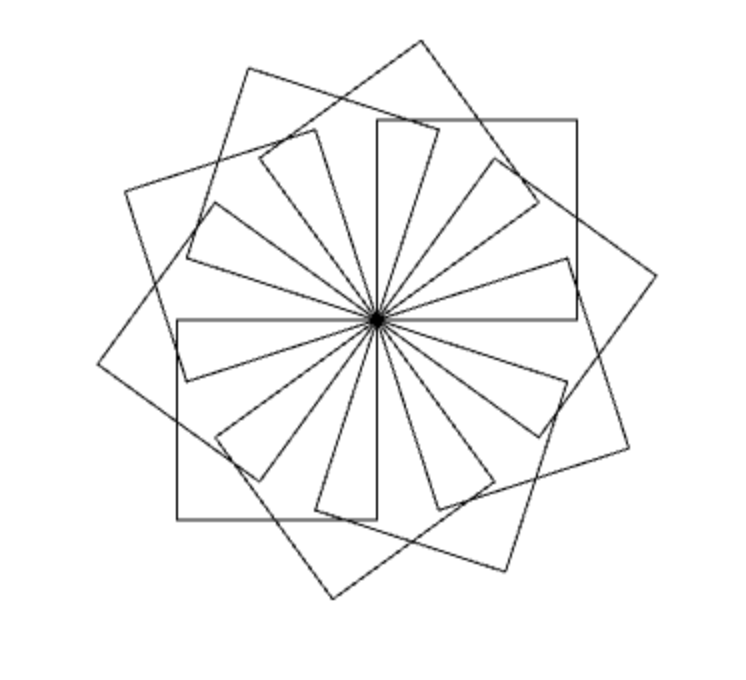
\includegraphics[width=0.2\pagewidth]{GrundlagenInfo/00_Programmieren/Figures/viereck_blume}
	\end{figure}
\end{frame}

\begin{frame}[fragile]{Schleifen in Schleifen}{Weitere Beispiele aus dem Buch}
	\begin{itemize}
		\item Beispiel 1.8
		\item Beispiel 1.9
	\end{itemize}
\end{frame}

\begin{frame}[fragile]{Auftrag}
	\begin{itemize}
		\item \aufgabebox{Buch, Aufgaben 1.15 bis 1.19}
		\item \abgabebox{Aufgabe 1.18: Abgabe auf Moodle}
	\end{itemize}
\end{frame}

\begin{frame}[fragile]{Datentypen}
	\begin{table}[H]
		\footnotesize
		\centering
		\begin{tabular}{l|p{2cm}|p{2cm}}
			\textbf{Beispiel}                                        & \textbf{Datentyp (englisch, Abk.)} & \textbf{Datentyp (Deutsch)} \\\midrule\midrule
			\lstinline|"Hallo Welt", "abc", "42"| & string (str)                       & Zeichenkette                \\\midrule
			\lstinline|15, 45, -5, 0|             & integer (int)                      & Ganzzahl                    \\\midrule
			\lstinline|12.23, -5.33, 23.0|        & float (float)                      & Kommazahl
		\end{tabular}
	\end{table}

	\textbf{Analogie}:
	\begin{itemize}
		\item Name (string)
		\item Alter in Jahren (integer)
		\item Grösse in Metern (float)
	\end{itemize}
\end{frame}

\begin{frame}[fragile]{Auftrag}
	\begin{itemize}
		\item \aufgabebox{Buch, Aufgaben 1.20 bis 1.28}
		\item \abgabebox{Aufgabe 1.20: Abgabe auf Moodle}
		\item Tipp: Backslash (\textbackslash)
		      \begin{itemize}
			      \item auf MacOS: \keys{\shift+\Alt+7}
			      \item auf Windows: \keys{\AltGr+\textbackslash}
		      \end{itemize}
	\end{itemize}
\end{frame}
